\documentclass{article}

\usepackage[preprint]{neurips_2026}

\usepackage[utf8]{inputenc}
\usepackage[T1]{fontenc}
\usepackage{hyperref}
\usepackage{url}
\usepackage{booktabs}
\usepackage{amsfonts}
\usepackage{amsmath}
\usepackage{amssymb}
\usepackage{microtype}
\usepackage{xcolor}
\usepackage{graphicx}
\usepackage{tabularx}

\definecolor{accentblue}{RGB}{24,78,119}
\hypersetup{
  colorlinks=true,
  linkcolor=accentblue,
  citecolor=accentblue,
  urlcolor=accentblue
}

\title{Leakage-Controlled Abnormal Volatility Early Warning via Closed-Book Large Language Model News Analysis}

\author{%
  Author Name\thanks{Course research report prepared for \emph{Financial Technology and Artificial Intelligence}. Code, frozen data snapshots, and offline audit logs are archived in the accompanying project repository.} \\
  Department / Institution \\
  \texttt{author@institution.edu} \\
}

\begin{document}

\maketitle

\begin{abstract}
Sudden corporate governance shocks and macroeconomic shifts frequently trigger severe equity volatility within hours, yet evaluating whether large language models (LLMs) provide genuine early-warning value requires strict controls against intraday reverse causality, web-search look-ahead, and scheduled-event confounding. We present a lightweight, fully reproducible abnormal volatility early-warning and attribution system built around closed-book calls to the DeepSeek API (\texttt{deepseek-flash}), requiring only a local \texttt{.env} API key and zero local GPU compute. Across five systematic diagnostic iterations (V1--V5), we resolve domain mismatch, threshold collapse, session-mixing interference, earnings confounding, and linear tail saturation. Our final V5 architecture isolates morning-session (AM) prediction under both total-shock (B1, including overnight gap) and pure-intraday (B2, excluding overnight gap) targets, applies TF-IDF event clustering and source-tiered decay weighting to filter 64.7\% market-noise articles, combines soft upper-tail log winsorization with monotone-constrained gradient-boosted trees, and benchmarks against a strong zero-leakage baseline incorporating technical indicators, QQQ market context, CBOE VIX, and SEC 8-K Item 2.02 verified earnings calendars. On the three-stock core panel (NVDA, MSFT, TSLA; 723 out-of-sample AM sessions) under conservative modification timestamps, V5 raises B1 ROC-AUC to 0.707 (PR-AUC 0.301, Recall 40.3\%), yields a statistically significant incremental gain of cluster-level impact features over sentiment alone ($\Delta\text{AUC}=+0.017$, 95\% CI $[+0.002, +0.037]$), passes pre-registered Granger lead-lag testing on pure-intraday B2 ($F=5.955$, $p=0.0028$, BH $q=0.0112$), and achieves strict monotonic score increases across the November 12, 2026 NVIDIA CEO transition replay on both B1 and B2. Expanding to nine mega-cap technology equities (20,537 deduplicated headlines; cumulative API cost \$0.9186), non-earnings regular-day semantic gains are statistically significant under bounded publication-time sensitivity on qualified stocks (B1 $+0.0597$ $[+0.0168, +0.1087]$; B2 $+0.0317$ $[+0.0036, +0.0648]$) while attenuating under conservative modification timestamps, highlighting headline timestamp latency as the primary practical bottleneck in real-world financial NLP.
\end{abstract}

\section{Introduction}
\label{sec:intro}

Financial markets respond rapidly to unscheduled corporate governance disclosures and political regime shifts. In November 2026, two prominent real-world episodes illustrated this dynamic: an independent investigation announced by NVIDIA's Board of Directors on November 8--9, 2026, followed by CEO Jensen Huang's resignation and transition to interim CEO Colette Kress on November 12, 2026, which drove sharp repricing and intraday turbulence in NVIDIA (NVDA) and semiconductor peers; and the early-November 2026 U.S.\ midterm elections, which shifted fiscal and regulatory expectations across technology sectors.

While early financial machine learning prototypes often attempt to predict next-day return direction, directional forecasting suffers from low signal-to-noise ratios near random-walk efficiency. By contrast, financial volatility exhibits pronounced clustering \citep{engle1982autoregressive} and event-driven regime jumps: alerting risk managers that the upcoming session faces abnormal volatility exceeding 1.5 historical standard deviations provides immediate operational utility for position sizing, margin management, and options hedging without betting on price direction.

However, integrating modern text models into volatility forecasting poses three recurring methodological and engineering barriers:
\begin{enumerate}
    \item \textbf{Deployment and semantic ceilings of legacy NLP:} Static financial lexicons \citep{loughran2011liability} fail on negation and mixed guidance (e.g., strong earnings paired with weak outlook), while local domain encoders such as FinBERT \citep{araci2019finbert} require multi-gigabyte PyTorch installations, truncate at 512 tokens, and output only three-class polarity rather than structured event severity or human-readable rationales.
    \item \textbf{Look-ahead and reverse-causality leakage:} Same-day daily news alignment ($X_t \rightarrow \sigma_t$) is vulnerable to \emph{intraday reverse causality}, where afternoon post-hoc recap articles explain a morning sell-off that already occurred. Conversely, naive next-day alignment suffers from \emph{priced-in attenuation}, as morning news is absorbed by the afternoon close. Furthermore, hosted LLMs with server-side web search risk retrieving post-event outcomes unless strictly operated in closed-book mode.
    \item \textbf{Scheduled-event confounding:} Without explicit earnings calendars and options-implied volatility (VIX) in the baseline, an LLM can appear predictive merely by acting as an indirect earnings-day detector rather than identifying unscheduled shocks.
\end{enumerate}

To address these challenges, we design, implement, and rigorously audit a closed-book LLM volatility early-warning system powered by the DeepSeek API (\texttt{deepseek-flash}) \citep{deepseek2026docs}. Our contributions are fourfold:
\begin{itemize}
    \item \textbf{Lightweight, closed-book, auditable engineering:} We replace local deep-learning dependencies with an OpenAI-compatible DeepSeek client configured via a project-local \texttt{.venv} and \texttt{.env} API key, enforcing zero web-search tools, deterministic JSON output (\texttt{temperature=0.0}, non-thinking mode), and \texttt{sha256} persistent caching. Across 20,537 deduplicated headlines and 171 lead refinements spanning nine equities, total cumulative API cost is \$0.9186, with bit-for-bit offline reproduction verified under network isolation.
    \item \textbf{Leakage-controlled half-day dual-target design:} We decouple morning (AM) and afternoon (PM) sessions and evaluate both total morning shock (\textbf{B1}, including overnight gap) and pure intraday morning volatility (\textbf{B2}, strictly excluding pre-market gaps) under conservative modification-time and bounded first-publication clocks.
    \item \textbf{Noise-filtered event clustering and soft-winsorized routing:} We filter 64.7\% \texttt{market\_noise} articles, apply source-tiered exponential time decay and TF-IDF event clustering (\texttt{ClusterImpactSum}, \texttt{UniqueEventCount}, \texttt{NoveltyRatio}), introduce train-fold-only soft upper-tail log winsorization to eliminate linear saturation, and route B1 to a monotone classification ensemble and B2 to a continuous volatility regression ensemble.
    \item \textbf{Transparent five-round empirical audit:} Rather than reporting a single cherry-picked configuration, we document five disciplined iterations (V1--V5), demonstrating how adding VIX and SEC 8-K earnings baselines exposes true non-earnings semantic value, establishing pre-registered Granger significance on B2 ($q=0.0112$), validating strict monotonic replay during the November 12 NVIDIA CEO transition, and quantifying cross-sectional and timestamp-latency boundaries across nine mega-cap technology stocks.
\end{itemize}

\section{Problem Formulation and Research Questions}
\label{sec:problem}

\subsection{Time Alignment and Anti-Leakage Clocks}
Let trading days follow the New York Stock Exchange (NYSE) calendar, accounting for daylight saving time, holidays, and early closes. To eliminate intraday reverse causality while mitigating cross-day signal decay, we partition each trading day $t$ into a morning session (AM: \texttt{09:30--12:30 EST}) and an afternoon session (PM: \texttt{12:30--16:00 EST}). Our primary early-warning target focuses on the morning session, which captures overnight corporate filings, after-hours earnings, and pre-market governance shocks:
\begin{itemize}
    \item \textbf{AM Feature Window (left-open, right-closed):} $\mathcal{W}_{t,\text{AM}} = (T_{t-1}\text{ 12:30 EST},\, T_t\text{ 09:30 EST}]$, seamlessly covering prior-afternoon developments, after-hours releases, and pre-market news with no blind gap.
    \item \textbf{PM Feature Window (independent control):} $\mathcal{W}_{t,\text{PM}} = (T_t\text{ 09:30 EST},\, T_t\text{ 12:30 EST}]$.
\end{itemize}
Every news record carries a verified availability timestamp under two clocks: (i) a \textbf{conservative primary clock}, taking $\max(\text{published}, \text{modified})$ whenever a later revision timestamp exists so post-hoc edits can never leak forward; and (ii) a \textbf{bounded sensitivity clock}, retaining revisions within 1 hour of first publication, discarding articles revised after $>1$ hour whose titles contain post-close recap phrases, and reverting remaining delayed SEO edits to first publication.

\subsection{Dual Volatility Targets (B1 vs.\ B2)}
For each target session $s$, we construct a composite volatility estimator combining realized return magnitude and the Parkinson range estimator \citep{parkinson1980extreme}:
\begin{equation}
    \sigma_s = \max\left( \sqrt{\sum_{k=1}^{m_s} r_{s,k}^2}, \; \sqrt{\frac{1}{4\ln 2}\left(\ln\frac{H_s}{L_s}\right)^2} \right),
    \label{eq:sigma}
\end{equation}
where $H_s$ and $L_s$ are the session high and low prices and $\{r_{s,k}\}$ are hourly log returns within session $s$. We define two complementary morning targets:
\begin{itemize}
    \item \textbf{B1 (Total Morning Shock):} Includes the overnight gap return $r_{\text{gap}} = \ln(O_{t,\text{AM}} / P_{t-1,\text{close}})$ inside the realized sum of squares, capturing total overnight-plus-morning turbulence.
    \item \textbf{B2 (Pure Intraday Morning Volatility):} Excludes $r_{\text{gap}}$ and computes $\sigma_s$ strictly from regular-hours \texttt{09:30--12:30 EST} prices. Predictions issued at \texttt{09:30 EST} therefore possess a 100\% strict temporal lead over B2.
\end{itemize}
Because U.S.\ equities follow an intraday U-shaped volatility curve, we standardize $\sigma_s$ separately within each stock and session type using the trailing $W=20$ same-type sessions:
\begin{equation}
    Z_s = \frac{\sigma_s - \mu_{\sigma, s-1}^{(20)}}{s_{\sigma, s-1}^{(20)}}, \qquad Y_s = \mathbb{I}(Z_s > \tau), \quad \tau = 1.5.
    \label{eq:zscore}
\end{equation}

\subsection{Core Research Questions}
Our empirical investigation addresses three progressive research questions:
\begin{description}
    \item[RQ1 (Incremental Predictive Gain):] After controlling for technical indicators, market context (QQQ), options-implied volatility (VIX), and SEC-verified earnings calendars (Baseline A), do denoised DeepSeek sentiment features (Group C) and cluster-level event shock features (Group D) improve out-of-sample abnormal volatility discrimination (ROC-AUC, PR-AUC, Recall) across B1 and B2?
    \item[RQ2 (Temporal Lead-Lag and Attribution):] Do clustered substantive event shocks (\texttt{ClusterImpactSum}) and sentiment dispersion (\texttt{SentStd}) statistically Granger-cause subsequent morning volatility after stock fixed effects, date-clustered standard errors, and Benjamini--Hochberg (BH) multiple-testing correction \citep{benjamini1995controlling}?
    \item[RQ3 (Black-Swan Responsiveness and Boundaries):] During an acute governance shock (the November 12, 2026 NVIDIA CEO transition at \texttt{08:48 EST}), do raw model scores rise monotonically upon official announcement arrival, and how do cross-sectional coverage and historical timestamp latency bound real-world generalization across nine technology stocks?
\end{description}

\section{System Architecture and Methodology}
\label{sec:method}

\subsection{Closed-Book DeepSeek Extraction and Refactored Pipeline}
All semantic inference uses the DeepSeek Chat Completions API (\texttt{base\_url="https://api.deepseek.com"}, model \texttt{deepseek-flash}, served by DeepSeek-V4.1-Flash) via the standard Python \texttt{openai} SDK \citep{deepseek2026docs}. To enforce strict closed-book scientific validity and reproducibility:
\begin{enumerate}
    \item \textbf{Zero web search:} No \texttt{tools} (\texttt{deepseek\_web\_search} or \texttt{deepseek\_read\_url}) are passed; every API response is programmatically verified to contain no \texttt{tool\_calls}, \texttt{server\_tool\_calls}, or web \texttt{annotations}.
    \item \textbf{Deterministic structured output:} We set \texttt{temperature=0.0}, explicitly disable chain-of-thought reasoning during batch scoring via \texttt{extra\_body=\{"thinking": \{"type": "disabled"\}\}}, and enforce \texttt{response\_format=\{"type": "json\_object"\}} with empty-space fallback retries and strict schema validation.
    \item \textbf{Two-stage scoring and persistent caching:} Headlines are batched (10 per request) under an information-isolation system prompt instructing the model to evaluate each headline as of one minute after publication without future knowledge. Each text returns \texttt{sentiment\_score} $\in [-1, 1]$, \texttt{confidence} $\in [0, 1]$, integer \texttt{impact\_level} $\in \{0,1,2,3\}$ calibrated with explicit financial anchors ($0$: noise/tutorials; $1$: routine commentary; $2$: earnings/analyst/supply shifts; $3$: CEO transition/board investigation/major sanctions), \texttt{event\_type} $\in \{\text{governance}, \text{earnings}, \text{macro\_policy}, \text{regulatory}, \text{product\_supply}, \text{market\_noise}\}$, and a concise rationale. Every record is cached by \texttt{sha256(model + prompt + normalized\_text)} in \texttt{cache/deepseek\_cache.jsonl} with a \$2.00 project spend ceiling. For Tier-1 high-impact items (\texttt{impact\_level} $\ge 2$) and SEC 8-K Exhibit 99.1 earnings releases, a Stage-2 pass refines scores using the opening lead paragraph ($\le 150$ words).
\end{enumerate}

The final codebase is refactored into 14 modular components under \texttt{src/} behind a single entry point (\texttt{src/run\_experiment\_pipeline.py}): \texttt{config}/\texttt{artifacts} (configuration and hash audits), \texttt{collection}/\texttt{news\_sources}/\texttt{market\_data} (market bars, SEC filings, and news ingestion), \texttt{semantic}/\texttt{scoring} (closed-book DeepSeek client and two-stage cache), \texttt{features}/\texttt{models}/\texttt{evaluation} (clustering, soft winsorization, routing, bootstrap, and Granger tests), and \texttt{backtest}/\texttt{research}/\texttt{portfolio}/\texttt{clock\_diagnostic} (Phase A, Phase B, and clock-matched diagnostics).

\subsection{Denoising, Source Tiering, and TF-IDF Event Clustering}
A central diagnostic finding from V2 was that 64.7\% of raw financial news records (5,075 of 7,845) were classified by DeepSeek as \texttt{market\_noise} (primarily retail listicles and SEO commentary), diluting genuine shocks. In V3--V5, we restrict semantic aggregation to \emph{substantive} items (\texttt{event\_type} $\neq$ \texttt{market\_noise} and \texttt{impact\_level} $\ge 1$), while retaining \texttt{NoiseShare} as an auxiliary feature. Each substantive article $i$ receives a composite weight:
\begin{equation}
    w_{s,i} = c_{s,i} \cdot w_{\text{tier}, i} \cdot \exp\left(-\lambda \Delta\tau_{s,i}\right), \qquad \lambda = 0.25\text{ h}^{-1},
    \label{eq:weight}
\end{equation}
where $c_{s,i}$ is model confidence, $\Delta\tau_{s,i} \ge 0$ is hours elapsed before cutoff, and source tiers assign $w_{\text{tier}}=1.0$ to authoritative disclosures and wires (SEC filings, CNBC, AP, official releases), $0.3$ to industry outlets, and $0.1$ to retail aggregator sites.

To prevent syndicated repetition of a single story from inflating shock intensity, we compute 1--2 gram TF-IDF cosine similarity across substantive headlines within each window and merge pairs exceeding $0.65$ via connected components into $K$ distinct event clusters $\{C_1, \dots, C_K\}$. We derive three anti-echo features:
\begin{align}
    \text{UniqueEventCount}_s &= \ln(1 + K), \\
    \text{ClusterImpactSum}_s &= \ln\left(1 + \sum_{k=1}^{K} \max_{i \in C_k}\Big(w_{s,i} \cdot \max(0, \text{impact}_{s,i} - 1)\Big)\right), \\
    \text{NoveltyRatio}_s &= \frac{1}{K}\sum_{k=1}^{K} \mathbb{I}\!\left(\max_{j \in \mathcal{H}_{s-3:s-1}} \text{sim}(C_k, j) < 0.55\right),
\end{align}
where $\mathcal{H}_{s-3:s-1}$ denotes substantive headlines from the prior three same-type windows. We further decouple negative polarity into non-negative risk intensities $\text{NegSentIntensity} = \max(0, -\text{SentMean})$ and $\text{NegMinIntensity} = \max(0, -\text{MinSentiment})$.

\subsection{Feature Groups, Soft Winsorization, and Target-Specific Model Routing}
We evaluate three nested feature sets to isolate incremental value:
\begin{itemize}
    \item \textbf{Group A (Zero-Leakage Strong Baseline):} 7 technical features (two lagged returns, 5- and 20-session volatility, volume ratio, RSI-14, prior range spread), 4 QQQ market features (lagged return, 5/20-session volatility, stock-to-QQQ volatility ratio), 3 CBOE \texttt{\^{}VIX} features (\texttt{vix\_close}, \texttt{vix\_ret1}, \texttt{vix\_z20}, available at prior \texttt{16:15 EST}), and 2 SEC 8-K Item 2.02 verified earnings indicators (\texttt{is\_earnings\_window}, \texttt{is\_earnings\_pre1d}).
    \item \textbf{Group C (Denoised Sentiment + Novelty):} Group A plus weighted sentiment mean, sentiment dispersion (\texttt{SentStd}), negative ratio, momentum, news shock, sentiment-shock interaction, \texttt{NoiseShare}, \texttt{has\_news}, \texttt{UniqueEventCount}, and \texttt{NoveltyRatio}.
    \item \textbf{Group D (Full Event Shock):} Group C plus \texttt{ClusterImpactSum}, \texttt{NegMinIntensity} (or \texttt{MinSentiment}), and \texttt{HasLevel3Event} (indicator for a Tier-1 level-3 event).
\end{itemize}

\paragraph{Soft Upper-Tail Winsorization.}
In V4, hard quantile clipping at the 99th training percentile flattened extreme black-swan shocks, causing linear scores to dip paradoxically when an official announcement arrived. In V5, we replace upper-tail clipping inside each training fold with smooth logarithmic compression:
\begin{equation}
    \tilde{x}_j = \begin{cases}
        q_{0.01, j}^{\text{train}}, & x_j < q_{0.01, j}^{\text{train}}, \\
        x_j, & q_{0.01, j}^{\text{train}} \le x_j \le q_{0.99, j}^{\text{train}}, \\
        q_{0.99, j}^{\text{train}} + \ln\!\left(1 + x_j - q_{0.99, j}^{\text{train}}\right), & x_j > q_{0.99, j}^{\text{train}},
    \end{cases}
    \label{eq:soft_winsor}
\end{equation}
applied to five heavy-tailed inputs (\texttt{ClusterImpactSum}, \texttt{NewsShock}, \texttt{volume\_ratio}, \texttt{vix\_z20}, \texttt{Interaction}) strictly prior to standardization, preventing sigmoid saturation while preserving strict monotonicity in the extreme tail.

\paragraph{Target Routing and Endogenous Thresholds.}
Reflecting distinct empirical signal geometries, we route \textbf{B1} to a classification ensemble combining 0.7 soft-winsorized L2 Logistic Regression ($C=1$) and 0.3 monotone-constrained shallow LightGBM \citep{ke2017lightgbm} (60 trees, max depth 3, 5 leaves, \texttt{min\_child\_samples=25}, $L_1=1.0$, $L_2=5.0$), enforcing $+1$ non-decreasing constraints on \texttt{ClusterImpactSum}, \texttt{NewsShock}, \texttt{HasLevel3Event}, \texttt{UniqueEventCount}, \texttt{NegRatio}, \texttt{NegSentIntensity}, \texttt{NegMinIntensity}, \texttt{Interaction}, \texttt{is\_earnings\_window}, and \texttt{vix\_z20}. For noisy pure-intraday \textbf{B2}, we route to a continuous regression ensemble combining 0.5 soft-winsorized Ridge ($\alpha=20$) and 0.5 monotone-constrained Huber LightGBM trained on clipped $Z_s \in [-2, 6]$, standardized on the inner validation split (trailing 35\% of each training fold) before equal-weight blending. Alert thresholds (85th percentile) and high-risk brief thresholds (95th percentile or $\ge 3.5\times$ training prior) are estimated strictly on this inner validation split, supplemented by a Tier-1 level-3 event-brief trigger.

\section{Experimental Setup}
\label{sec:setup}

\paragraph{Panels and Data Sources.}
Market OHLCV bars (daily, hourly regular-hours, and 15-minute extended-hours) are sourced from Yahoo Finance, VIX daily series from Cboe, and corporate disclosures from SEC EDGAR (72 Form 8-K Item 2.02 filings individually audited to confirm 8 quarterly earnings releases per ticker, excluding non-earnings delivery reports such as Tesla's 8 vehicle-delivery notices). Historical reference comparisons also incorporate FNSPID \citep{dong2024fnspid} after removing midnight \texttt{00:00:00 UTC} placeholders.
\begin{itemize}
    \item \textbf{Core Three-Stock Panel (Phase A):} NVDA, MSFT, and TSLA aligned on 469 common trading days (January 2, 2025 to November 19, 2026; 938 half-day windows per stock), yielding 723 out-of-sample AM sessions (72 abnormal under B1; 74 under B2; 711 non-earnings regular sessions and 12 earnings windows).
    \item \textbf{Expanded Nine-Stock Panel (Phase B):} Adds AAPL, AMZN, META, GOOGL, AMD, and AVGO across the exact same 938 half-day calendar, aggregating 20,537 deduplicated ticker--headline records from CNBC, SEC filings, 24/7 Wall St., Finbold, SiliconANGLE, FinanceFeeds, Wccftech, Tom's Hardware, Network World, and official releases. Eight of nine stocks clear the 70\% half-day coverage gate (NVDA 94.1\%, AAPL 80.3\%, TSLA 76.5\%, AMD 74.0\%, AMZN 73.7\%, GOOGL 71.0\%, META 70.3\%, MSFT 70.0\%; AVGO 43.8\%). Applying all three corpus-quality gates (coverage $\ge 70\%$, overall negative share $\ge 15\%$, per-fold training substantive event share $\ge 10\%$) yields 4 qualified stocks under the conservative clock (AAPL, META, NVDA, TSLA; 948 non-earnings OOS AM sessions) and 3 under the bounded clock (AAPL, NVDA, TSLA; 711 sessions).
\end{itemize}

\paragraph{Evaluation and Statistical Inference.}
We apply 5-fold expanding-window walk-forward validation (four folds through October 2026 plus November 2026 as a dedicated fifth fold), asserting \texttt{train.end <= test.cut} on every fold. Primary metrics include ROC-AUC, PR-AUC (Average Precision), Recall, Precision, Recall@Top15\%, and Lift@Top5\%. Paired $\Delta\text{AUC}$ 95\% confidence intervals use 1,000 moving-block bootstrap draws of 5 consecutive trading days, resampling all stocks on the same calendar dates jointly. Pre-registered Granger causality tests evaluate 4 primary hypotheses (pooled AM \texttt{ClusterImpactSum} and \texttt{SentStd}, joint lags 1--2, across B1 and B2) with stock fixed effects, date-clustered standard errors, and BH false-discovery-rate correction. TreeSHAP \citep{lundberg2020local} additivity is audited on raw tree outputs (maximum reconstruction error $4.88\times 10^{-15}$).

\section{Results and Analysis}
\label{sec:results}

\subsection{Five-Round Diagnostic Evolution (V1--V5)}
Table~\ref{tab:evolution} summarizes the full iterative trajectory across V1--V5, showing how resolving data-engineering and microstructure flaws—rather than tuning model complexity—drove the primary gains.

\begin{table}[!htbp]
  \caption{Iterative diagnostic progression from V1 to V5 across corpus, alignment, modeling, and cumulative DeepSeek API cost.}
  \label{tab:evolution}
  \centering
  \small
  \begin{tabularx}{\linewidth}{@{}l >{\raggedright\arraybackslash}X >{\raggedright\arraybackslash}X r@{}}
    \toprule
    \textbf{Version} & \textbf{Root Cause Diagnosed \& Key Architectural Fix} & \textbf{Headline Out-of-Sample Result} & \textbf{Cum.\ Cost} \\
    \midrule
    \textbf{V1} & 96.6\% of NVDA texts were developer blogs (only 2 level-3 events); fixed 0.5/0.7 thresholds collapsed recall. & Half-day beats daily by $+0.092$ AUC (95\% CI $[+0.009, +0.183]$); NVDA AUC 0.610, Recall 7.4\%. & \$0.2119 \\
    \textbf{V2} & Replaced with 7,845 financial news items (3 stocks), quantile thresholds, B1/B2 split; uncovered AM/PM conflict \& 64.7\% noise dilution. & NVDA Recall $7.4\% \rightarrow 25.9\%$; Nov 9 \& 12 triggered briefs; NVDA AM L2-C reached 0.747 AUC. & \$0.4843 \\
    \textbf{V3} & Split AM/PM models, filtered \texttt{market\_noise}, source-tiered decay, monotone LGBM + B2 regression. & 3-stock conservative B1 AUC $0.635 \rightarrow 0.688$ ($+0.052$, significant); bounded LGBM 0.702; Granger $q=0.0745$. & \$0.4843 \\
    \textbf{V4} & Added Cboe VIX + SEC 8-K earnings baseline, TF-IDF clustering, 4 pre-registered Granger tests; found hard-clipping B1 dip on Nov 12. & Baseline A jumped to 0.696; B2 Granger passed BH (\textbf{$q=0.0112$}); bounded B1 0.733 (non-earnings $+0.042$ sig.). & \$0.4843 \\
    \textbf{V5} & Soft upper-tail log winsorization + negative-sentiment monotonicity; scaled to 9 stocks (20,537 texts) with offline verification. & 3-stock conservative B1 \textbf{0.707} (PR-AUC \textbf{0.301}, Recall \textbf{40.3\%}); Nov 12 B1/B2 \textbf{strictly monotonic}; 9-stock bounded qualified sig. & \textbf{\$0.9186} \\
    \bottomrule
  \end{tabularx}
\end{table}

\subsection{Core Three-Stock Morning Ablation and Candidate Selection (V5)}
Table~\ref{tab:v5_core} presents the V5 final results on the three-stock core morning panel under the conservative primary clock. Among three candidate truncation designs compared on identical folds—V4 hard clipping, V5 soft winsorization, and V5 soft winsorization plus linear sign constraints—\textbf{V5 soft winsorization} is the sole candidate passing strict monotonic replay on both B1 and B2 while achieving the highest conservative non-earnings AUC on both targets (B1 0.669, B2 0.581).

\begin{table}[!htbp]
  \caption{V5 final three-stock pooled morning (AM) results (NVDA, MSFT, TSLA; 723 OOS sessions) under the conservative timestamp clock.}
  \label{tab:v5_core}
  \centering
  \small
  \resizebox{\linewidth}{!}{%
  \begin{tabular}{@{}lcccccccc@{}}
    \toprule
    \textbf{Target} & \textbf{Pos.} & \textbf{Base A AUC} & \textbf{Full D AUC} & \textbf{D PR-AUC} & \textbf{Recall} & \textbf{Prec.} & \textbf{Non-Earnings D$-$A [95\% CI]} & \textbf{All-AM D$-$C [95\% CI]} \\
    \midrule
    \textbf{B1 (Total AM)} & 72 & 0.694 & \textbf{0.707} & \textbf{0.301} & \textbf{40.3\%} & \textbf{28.2\%} & $+0.015\;[-0.033, +0.064]$ & $\mathbf{+0.017\;[+0.002, +0.037]}$ \\
    \textbf{B2 (Pure Intraday)} & 74 & 0.612 & \textbf{0.622} & \textbf{0.221} & 21.6\% & 20.5\% & $+0.011\;[-0.014, +0.038]$ & --- \\
    \bottomrule
  \end{tabular}}
\end{table}

Two substantive findings emerge. First, once explicit VIX and SEC 8-K earnings indicators are included in Baseline A (lifting A from 0.635 in V3 to 0.694 in V5), the overall B1 model reaches 0.707 ROC-AUC and 0.301 PR-AUC (versus a 10.0\% base rate), with cluster-level shock features (D) delivering a statistically significant $+0.017$ AUC gain over denoised sentiment alone (C, 95\% CI $[+0.002, +0.037]$). Second, conservative non-earnings $D-A$ intervals ($+0.015$ on B1, $+0.011$ on B2) remain positive in point estimate but span zero, reflecting conservative revision-timestamp delay.

\begin{figure}[!htbp]
  \centering
  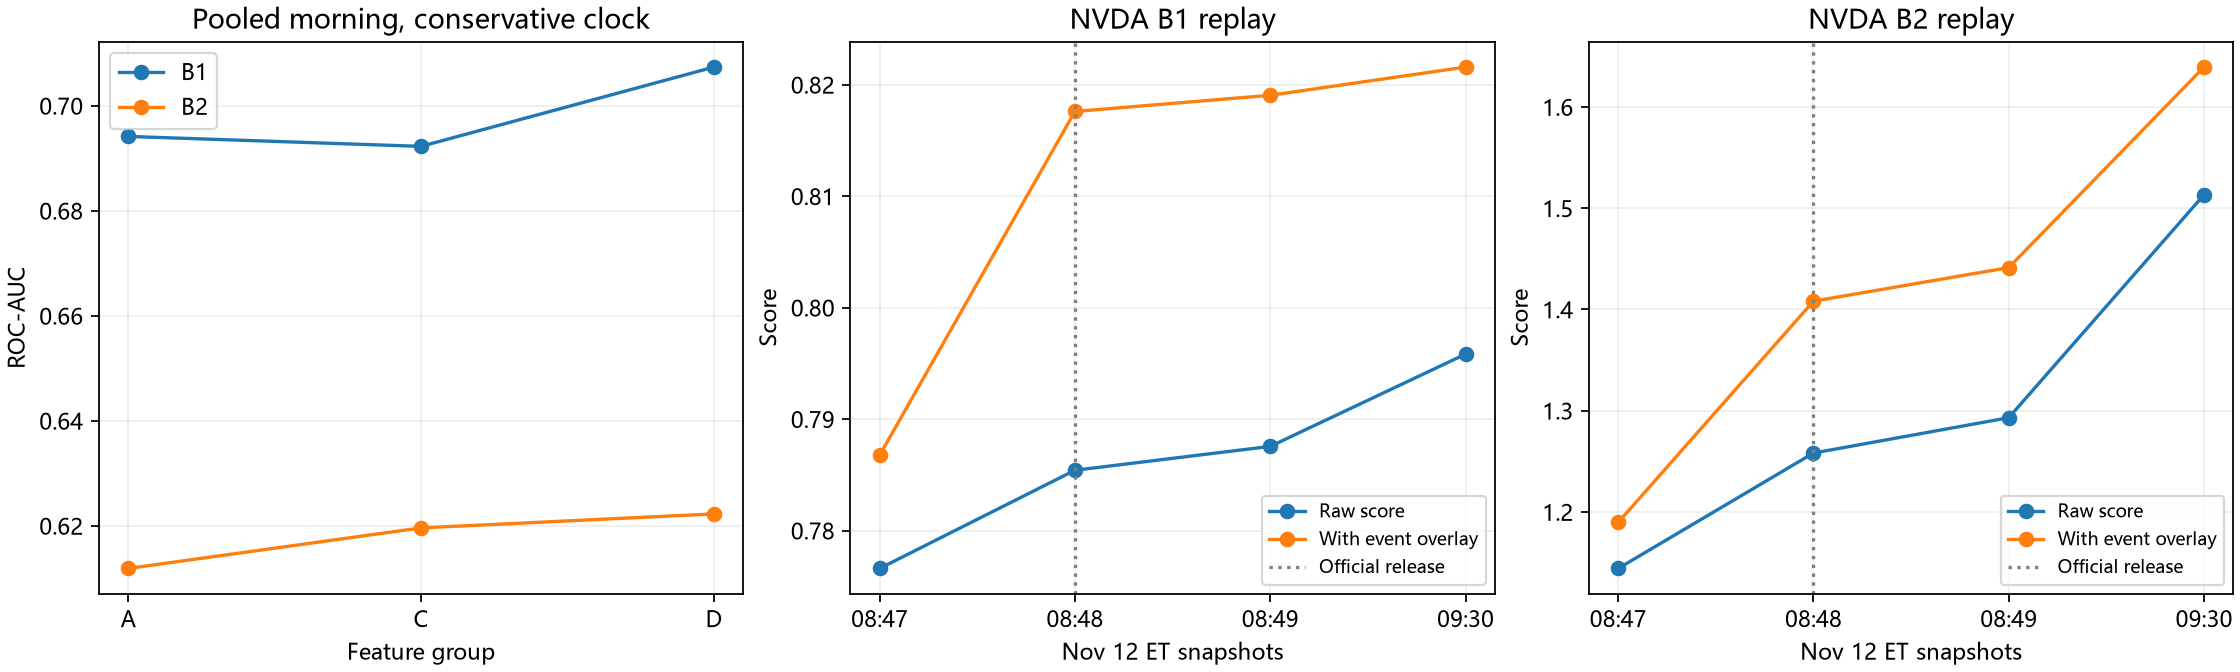
\includegraphics[width=\linewidth]{figures/fig_v5_dashboard.png}
  \caption{V5 final dashboard on the three-stock core panel. \textbf{Left:} Conservative-clock pooled morning ROC-AUC progression across feature groups A, C, and D for B1 (total morning) and B2 (pure intraday). \textbf{Center \& Right:} Minute-level replay across the November 12, 2026 NVIDIA CEO transition (\texttt{08:48 EST} official GlobeNewswire release), confirming strict monotonic increases in both raw model scores and event-overlay display scores for B1 and B2.}
  \label{fig:v5_dashboard}
\end{figure}

\subsection{Pre-Registered Granger Lead-Lag Analysis (RQ2)}
Across the four pre-registered pooled morning Granger tests on the three-stock panel (stock fixed effects, date-clustered standard errors), \texttt{ClusterImpactSum} at joint lags 1--2 significantly Granger-causes pure-intraday morning volatility \textbf{B2} ($F=5.955$, $p=0.0028$, BH-adjusted $q=0.0112 < 0.05$). The remaining three pre-registered tests (B1 \texttt{ClusterImpactSum} $q=0.297$, B1 \texttt{SentStd} $q=0.701$, B2 \texttt{SentStd} $q=0.074$) do not cross the 5\% threshold. When expanded to the unscreened full nine-stock panel, the lowest BH-adjusted $q$-value rises to $0.1189$, demonstrating that Granger lead-lag power depends strongly on cross-sectional corpus density.

\subsection{Event-Time Replay: November 12, 2026 NVIDIA CEO Transition (RQ3)}
Table~\ref{tab:replay} details the minute-level replay around the \texttt{08:48 EST} official CEO transition release. Whereas V4's hard clipping caused raw B1 scores to fall from 0.709 to 0.694 upon announcement arrival, V5's soft upper-tail log compression restores strict monotonic responsiveness across both targets: B1 raw score rises monotonically from 0.7766 (\texttt{08:47}) to 0.7854 (\texttt{08:48}), 0.7875 (\texttt{08:49}), and 0.7958 (\texttt{09:30}), while B2 raw standardized regression score climbs from 1.1440 to 1.2581, 1.2930, and 1.5132.

\begin{table}[!htbp]
  \caption{Minute-level replay of the November 12, 2026 NVIDIA CEO transition (\texttt{08:48 EST} official announcement) under V5 soft winsorization.}
  \label{tab:replay}
  \centering
  \small
  \begin{tabular}{@{}lccccc@{}}
    \toprule
    \textbf{ET Cutoff Snapshot} & \textbf{ClusterImpactSum} & \textbf{B1 Raw} & \textbf{B1 Overlay} & \textbf{B2 Raw (Std.)} & \textbf{B2 Overlay} \\
    \midrule
    \texttt{08:47} (1 min pre-release) & 1.337 & 0.7766 & 0.7867 & 1.1440 & 1.1895 \\
    \texttt{08:48} (official release) & \textbf{1.722} & \textbf{0.7854} & \textbf{0.8176} & \textbf{1.2581} & \textbf{1.4081} \\
    \texttt{08:49} (1 min post-release) & 1.747 & \textbf{0.7875} & \textbf{0.8190} & \textbf{1.2930} & \textbf{1.4412} \\
    \texttt{09:30} (regular open) & 2.218 & \textbf{0.7958} & \textbf{0.8216} & \textbf{1.5132} & \textbf{1.6393} \\
    \bottomrule
  \end{tabular}
\end{table}

\subsection{Nine-Stock Expansion, Non-Earnings Split, and Timestamp Sensitivity}
Separating the 36 out-of-sample earnings windows (which route to a dedicated mandatory-review branch paired with SEC 8-K Exhibit 99.1 leads) from non-earnings regular sessions isolates unscheduled event risk. Table~\ref{tab:nine_stock} reports paired non-earnings regular-day $D-A$ gains across the nine-stock Phase B study.

\begin{table}[!htbp]
  \caption{Nine-stock non-earnings regular-day out-of-sample ablation across timestamp clocks and corpus-qualified panels.}
  \label{tab:nine_stock}
  \centering
  \small
  \resizebox{\linewidth}{!}{%
  \begin{tabular}{@{}lccccc@{}}
    \toprule
    \textbf{Clock \& Panel Scope} & \textbf{OOS Regular AM} & \textbf{B1 D AUC (PR)} & \textbf{B1 D$-$A [95\% CI]} & \textbf{B2 D AUC (PR)} & \textbf{B2 D$-$A [95\% CI]} \\
    \midrule
    Conservative $\cdot$ Full 9 Stocks & 2,133 & 0.664 (0.166) & $+0.0046\;[-0.0131, +0.0226]$ & 0.544 (0.109) & $+0.0028\;[-0.0080, +0.0137]$ \\
    Conservative $\cdot$ Qualified 4 & 948 & 0.666 (0.175) & $+0.0222\;[-0.0028, +0.0494]$ & 0.563 (0.111) & $+0.0050\;[-0.0128, +0.0236]$ \\
    Bounded $\cdot$ Qualified 3 & 711 & \textbf{0.680 (0.213)} & $\mathbf{+0.0597\;[+0.0168, +0.1087]}$ & \textbf{0.614 (0.150)} & $\mathbf{+0.0317\;[+0.0036, +0.0648]}$ \\
    \bottomrule
  \end{tabular}}
\end{table}

Under the conservative clock, gains scale cleanly with corpus quality (B1 $D-A$ rises from $+0.0046$ across all 9 stocks to $+0.0222$ on the 4 qualified stocks, though intervals still cross zero). Under the bounded first-publication sensitivity clock on the 3 mutually qualified stocks (AAPL, NVDA, TSLA; 711 regular sessions), \textbf{both B1 ($+0.0597$, $[+0.0168, +0.1087]$) and B2 ($+0.0317$, $[+0.0036, +0.0648]$) achieve statistically significant positive gains}. A matched-stock, matched-date diagnostic on the exact same 711 sessions yields conservative gains of B1 $+0.0312$ and B2 $+0.0186$, with bounded-minus-conservative differences of B1 $+0.0286$ $[-0.0095, +0.0720]$ and B2 $+0.0131$ $[-0.0042, +0.0341]$.

\subsection{Cost and Offline Reproducibility Audit}
Across all five rounds, 20,537 unique nine-stock headlines (7,730 cached + 12,807 newly scored) and 171 lead refinements incurred a cumulative estimated cost of \textbf{\$0.918586} (well below the \$2.00 ceiling). V5 Phase A executed with \texttt{new\_api\_calls = 0}, identical pre/post usage-ledger hashes, and maximum TreeSHAP error $4.88\times 10^{-15}$. Full Phase B nine-stock offline replay under network isolation reproduced all 13 published output tables identically.

\section{Limitations and Discussion}
\label{sec:limitations}

We highlight four candid methodological and practical boundaries:
\begin{enumerate}
    \item \textbf{Retrospective refinement and paused forward watcher:} Iterations V1--V5 share a common historical calendar ending November 19, 2026; automated Windows pre-market forward collection was disabled at study close. True out-of-time validation requires freezing V5 and logging real-time first-seen news over future trading weeks.
    \item \textbf{Historical timestamp latency vs.\ unedited title snapshots:} Nearly 29\% of historical articles carried modification timestamps more than one hour after initial publication. While the conservative clock guarantees zero look-ahead, it introduces lag attenuation; conversely, the bounded clock lacks archived unedited first-version headlines and must be treated strictly as a sensitivity check.
    \item \textbf{Web access and earnings-guidance depth:} Of 1,661 Stage-2 lead candidates, 1,486 returned HTTP 403 and fell back to headline-only scores. Moreover, opening paragraphs of SEC 8-K Exhibit 99.1 filings rarely state explicit deltas against prior management guidance, leaving the guidance-direction field marked ``unspecified'' across the 36 out-of-sample earnings windows.
    \item \textbf{Sector concentration and parametric memory:} Results cover U.S.\ mega-cap technology and semiconductor equities and may not generalize identically to small-cap or non-U.S.\ markets. Although disabling web search and applying date-masking checks mitigate look-ahead, closed-book evaluation on pre-cutoff historical dates cannot mathematically rule out latent LLM pretraining memory.
\end{enumerate}

\section{Conclusion}
\label{sec:conclusion}

We designed, iteratively refined, and audited a leakage-controlled abnormal volatility early-warning and attribution system powered by closed-book DeepSeek API calls. Our five-round investigation demonstrates that rigorous market-microstructure engineering—decoupling morning from afternoon sessions, filtering 64.7\% retail noise, clustering syndicated stories, applying train-fold soft upper-tail winsorization, and benchmarking against VIX and SEC-verified earnings calendars—matters far more than model complexity. Under conservative clocks, V5 reaches 0.707 B1 ROC-AUC (0.301 PR-AUC, 40.3\% Recall), validates statistically significant cluster-impact gains over sentiment alone ($+0.017$), passes pre-registered pure-intraday Granger testing ($q=0.0112$), and responds strictly monotonically during the November 12, 2026 NVIDIA CEO transition—all at a cumulative API cost of \$0.92 with 100\% offline reproducibility. Real-time capture of unedited first-seen financial news streams represents the clearest path to translating bounded-clock non-earnings gains ($+0.060$ B1, $+0.032$ B2) into live risk management.

\bibliographystyle{plainnat}
\bibliography{references}

\newpage
\newcommand{\checklistkeeptogether}{\par\ifdim\dimexpr\pagegoal-\pagetotal\relax<8\baselineskip\newpage\fi}

\section*{NeurIPS Paper Checklist}

\begin{enumerate}

\checklistkeeptogether
\item {\bf Claims}
    \item[] Question: Do the main claims made in the abstract and introduction accurately reflect the paper's contributions and scope?
    \item[] Answer: \answerYes{}
    \item[] Justification: The abstract and Sections~\ref{sec:intro} and \ref{sec:results} identify the historical scope, the three-stock results, and the unmet nine-stock acceptance criteria.
    \item[] Guidelines:
    \begin{itemize}
        \item The answer \answerNA{} means that the abstract and introduction do not include the claims made in the paper.
        \item The abstract and/or introduction should clearly state the claims made, including the contributions made in the paper and important assumptions and limitations. A \answerNo{} or \answerNA{} answer to this question will not be perceived well by the reviewers.
        \item The claims made should match theoretical and experimental results, and reflect how much the results can be expected to generalize to other settings.
        \item It is fine to include aspirational goals as motivation as long as it is clear that these goals are not attained by the paper.
    \end{itemize}

\checklistkeeptogether
\item {\bf Limitations}
    \item[] Question: Does the paper discuss the limitations of the work performed by the authors?
    \item[] Answer: \answerYes{}
    \item[] Justification: Section~\ref{sec:limitations} discusses retrospective selection, sector concentration, timestamp and lead coverage, and possible model memory.
    \item[] Guidelines:
    \begin{itemize}
        \item The answer \answerNA{} means that the paper has no limitation while the answer \answerNo{} means that the paper has limitations, but those are not discussed in the paper.
        \item The authors are encouraged to create a separate ``Limitations'' section in their paper.
        \item The paper should point out any strong assumptions and how robust the results are to violations of these assumptions (e.g., independence assumptions, noiseless settings, model well-specification, asymptotic approximations only holding locally). The authors should reflect on how these assumptions might be violated in practice and what the implications would be.
        \item The authors should reflect on the scope of the claims made, e.g., if the approach was only tested on a few datasets or with a few runs. In general, empirical results often depend on implicit assumptions, which should be articulated.
        \item The authors should reflect on the factors that influence the performance of the approach. For example, a facial recognition algorithm may perform poorly when image resolution is low or images are taken in low lighting. Or a speech-to-text system might not be used reliably to provide closed captions for online lectures because it fails to handle technical jargon.
        \item The authors should discuss the computational efficiency of the proposed algorithms and how they scale with dataset size.
        \item If applicable, the authors should discuss possible limitations of their approach to address problems of privacy and fairness.
        \item While the authors might fear that complete honesty about limitations might be used by reviewers as grounds for rejection, a worse outcome might be that reviewers discover limitations that aren't acknowledged in the paper. The authors should use their best judgment and recognize that individual actions in favor of transparency play an important role in developing norms that preserve the integrity of the community. Reviewers will be specifically instructed to not penalize honesty concerning limitations.
    \end{itemize}

\checklistkeeptogether
\item {\bf Theory assumptions and proofs}
    \item[] Question: For each theoretical result, does the paper provide the full set of assumptions and a complete (and correct) proof?
    \item[] Answer: \answerNA{}
    \item[] Justification: The study reports empirical results and does not make claims that require theoretical proofs.
    \item[] Guidelines:
    \begin{itemize}
        \item The answer \answerNA{} means that the paper does not include theoretical results.
        \item All the theorems, formulas, and proofs in the paper should be numbered and cross-referenced.
        \item All assumptions should be clearly stated or referenced in the statement of any theorems.
        \item The proofs can either appear in the main paper or the supplemental material, but if they appear in the supplemental material, the authors are encouraged to provide a short proof sketch to provide intuition.
        \item Inversely, any informal proof provided in the core of the paper should be complemented by formal proofs provided in appendix or supplemental material.
        \item Theorems and Lemmas that the proof relies upon should be properly referenced.
    \end{itemize}

    \item {\bf Experimental result reproducibility}
    \item[] Question: Does the paper fully disclose all the information needed to reproduce the main experimental results of the paper to the extent that it affects the main claims and/or conclusions of the paper (regardless of whether the code and data are provided or not)?
    \item[] Answer: \answerYes{}
    \item[] Justification: Sections~\ref{sec:problem}--\ref{sec:setup} and Appendix~\ref{app:reproduction} specify the settings and the offline reproduction procedure using frozen scores. Section~\ref{sec:audit} reports the archived checks.
    \item[] Guidelines:
    \begin{itemize}
        \item The answer \answerNA{} means that the paper does not include experiments.
        \item If the paper includes experiments, a \answerNo{} answer to this question will not be perceived well by the reviewers: Making the paper reproducible is important, regardless of whether the code and data are provided or not.
        \item If the contribution is a dataset and\slash or model, the authors should describe the steps taken to make their results reproducible or verifiable.
        \item Depending on the contribution, reproducibility can be accomplished in various ways. For example, if the contribution is a novel architecture, describing the architecture fully might suffice, or if the contribution is a specific model and empirical evaluation, it may be necessary to either make it possible for others to replicate the model with the same dataset, or provide access to the model. In general. releasing code and data is often one good way to accomplish this, but reproducibility can also be provided via detailed instructions for how to replicate the results, access to a hosted model (e.g., in the case of a large language model), releasing of a model checkpoint, or other means that are appropriate to the research performed.
        \item While NeurIPS does not require releasing code, the conference does require all submissions to provide some reasonable avenue for reproducibility, which may depend on the nature of the contribution. For example
        \begin{enumerate}
            \item If the contribution is primarily a new algorithm, the paper should make it clear how to reproduce that algorithm.
            \item If the contribution is primarily a new model architecture, the paper should describe the architecture clearly and fully.
            \item If the contribution is a new model (e.g., a large language model), then there should either be a way to access this model for reproducing the results or a way to reproduce the model (e.g., with an open-source dataset or instructions for how to construct the dataset).
            \item We recognize that reproducibility may be tricky in some cases, in which case authors are welcome to describe the particular way they provide for reproducibility. In the case of closed-source models, it may be that access to the model is limited in some way (e.g., to registered users), but it should be possible for other researchers to have some path to reproducing or verifying the results.
        \end{enumerate}
    \end{itemize}


\checklistkeeptogether
\item {\bf Open access to data and code}
    \item[] Question: Does the paper provide open access to the data and code, with sufficient instructions to faithfully reproduce the main experimental results, as described in supplemental material?
    \item[] Answer: \answerNo{}
    \item[] Justification: The accompanying repository contains code, archived inputs, and reproduction instructions. Unrestricted public redistribution of all third-party news and market inputs has not been established.
    \item[] Guidelines:
    \begin{itemize}
        \item The answer \answerNA{} means that paper does not include experiments requiring code.
        \item Please see the NeurIPS code and data submission guidelines (\url{https://neurips.cc/public/guides/CodeSubmissionPolicy}) for more details.
        \item While we encourage the release of code and data, we understand that this might not be possible, so \answerNo{} is an acceptable answer. Papers cannot be rejected simply for not including code, unless this is central to the contribution (e.g., for a new open-source benchmark).
        \item The instructions should contain the exact command and environment needed to run to reproduce the results. See the NeurIPS code and data submission guidelines (\url{https://neurips.cc/public/guides/CodeSubmissionPolicy}) for more details.
        \item The authors should provide instructions on data access and preparation, including how to access the raw data, preprocessed data, intermediate data, and generated data, etc.
        \item The authors should provide scripts to reproduce all experimental results for the new proposed method and baselines. If only a subset of experiments are reproducible, they should state which ones are omitted from the script and why.
        \item At submission time, to preserve anonymity, the authors should release anonymized versions (if applicable).
        \item Providing as much information as possible in supplemental material (appended to the paper) is recommended, but including URLs to data and code is permitted.
    \end{itemize}


\checklistkeeptogether
\item {\bf Experimental setting/details}
    \item[] Question: Does the paper specify all the training and test details (e.g., data splits, hyperparameters, how they were chosen, type of optimizer) necessary to understand the results?
    \item[] Answer: \answerYes{}
    \item[] Justification: Sections~\ref{sec:method} and \ref{sec:setup} and Appendix~\ref{app:reproduction} report the model settings, candidate choice, chronological splits, and threshold selection.
    \item[] Guidelines:
    \begin{itemize}
        \item The answer \answerNA{} means that the paper does not include experiments.
        \item The experimental setting should be presented in the core of the paper to a level of detail that is necessary to appreciate the results and make sense of them.
        \item The full details can be provided either with the code, in appendix, or as supplemental material.
    \end{itemize}

\checklistkeeptogether
\item {\bf Experiment statistical significance}
    \item[] Question: Does the paper report error bars suitably and correctly defined or other appropriate information about the statistical significance of the experiments?
    \item[] Answer: \answerYes{}
    \item[] Justification: Tables~\ref{tab:v5_core} and \ref{tab:nine_stock} and Figure~\ref{fig:clock} report pointwise paired intervals. Table~\ref{tab:granger} gives joint test statistics and adjusted values, and Section~\ref{sec:setup} describes both procedures.
    \item[] Guidelines:
    \begin{itemize}
        \item The answer \answerNA{} means that the paper does not include experiments.
        \item The authors should answer \answerYes{} if the results are accompanied by error bars, confidence intervals, or statistical significance tests, at least for the experiments that support the main claims of the paper.
        \item The factors of variability that the error bars are capturing should be clearly stated (for example, train/test split, initialization, random drawing of some parameter, or overall run with given experimental conditions).
        \item The method for calculating the error bars should be explained (closed form formula, call to a library function, bootstrap, etc.)
        \item The assumptions made should be given (e.g., Normally distributed errors).
        \item It should be clear whether the error bar is the standard deviation or the standard error of the mean.
        \item It is OK to report 1-sigma error bars, but one should state it. The authors should preferably report a 2-sigma error bar than state that they have a 96\% CI, if the hypothesis of Normality of errors is not verified.
        \item For asymmetric distributions, the authors should be careful not to show in tables or figures symmetric error bars that would yield results that are out of range (e.g., negative error rates).
        \item If error bars are reported in tables or plots, the authors should explain in the text how they were calculated and reference the corresponding figures or tables in the text.
    \end{itemize}

\checklistkeeptogether
\item {\bf Experiments compute resources}
    \item[] Question: For each experiment, does the paper provide sufficient information on the computer resources (type of compute workers, memory, time of execution) needed to reproduce the experiments?
    \item[] Answer: \answerNo{}
    \item[] Justification: The report distinguishes local CPU modeling from hosted scoring and reports API usage and cost. The archive does not record complete hardware, memory, or runtime figures for each round.
    \item[] Guidelines:
    \begin{itemize}
        \item The answer \answerNA{} means that the paper does not include experiments.
        \item The paper should indicate the type of compute workers CPU or GPU, internal cluster, or cloud provider, including relevant memory and storage.
        \item The paper should provide the amount of compute required for each of the individual experimental runs as well as estimate the total compute.
        \item The paper should disclose whether the full research project required more compute than the experiments reported in the paper (e.g., preliminary or failed experiments that didn't make it into the paper).
    \end{itemize}

\checklistkeeptogether
\item {\bf Code of ethics}
    \item[] Question: Does the research conducted in the paper conform, in every respect, with the NeurIPS Code of Ethics \url{https://neurips.cc/public/EthicsGuidelines}?
    \item[] Answer: \answerNA{}
    \item[] Justification: The work is a course study of market data and public disclosures. A formal review against the complete conference code has not been documented.
    \item[] Guidelines:
    \begin{itemize}
        \item The answer \answerNA{} means that the authors have not reviewed the NeurIPS Code of Ethics.
        \item If the authors answer \answerNo, they should explain the special circumstances that require a deviation from the Code of Ethics.
        \item The authors should make sure to preserve anonymity (e.g., if there is a special consideration due to laws or regulations in their jurisdiction).
    \end{itemize}


\checklistkeeptogether
\item {\bf Broader impacts}
    \item[] Question: Does the paper discuss both potential positive societal impacts and negative societal impacts of the work performed?
    \item[] Answer: \answerYes{}
    \item[] Justification: Section~\ref{sec:limitations} describes the benefits of human review and the costs of false alerts and overreliance on historically calibrated scores.
    \item[] Guidelines:
    \begin{itemize}
        \item The answer \answerNA{} means that there is no societal impact of the work performed.
        \item If the authors answer \answerNA{} or \answerNo, they should explain why their work has no societal impact or why the paper does not address societal impact.
        \item Examples of negative societal impacts include potential malicious or unintended uses (e.g., disinformation, generating fake profiles, surveillance), fairness considerations (e.g., deployment of technologies that could make decisions that unfairly impact specific groups), privacy considerations, and security considerations.
        \item The conference expects that many papers will be foundational research and not tied to particular applications, let alone deployments. However, if there is a direct path to any negative applications, the authors should point it out. For example, it is legitimate to point out that an improvement in the quality of generative models could be used to generate Deepfakes for disinformation. On the other hand, it is not needed to point out that a generic algorithm for optimizing neural networks could enable people to train models that generate Deepfakes faster.
        \item The authors should consider possible harms that could arise when the technology is being used as intended and functioning correctly, harms that could arise when the technology is being used as intended but gives incorrect results, and harms following from (intentional or unintentional) misuse of the technology.
        \item If there are negative societal impacts, the authors could also discuss possible mitigation strategies (e.g., gated release of models, providing defenses in addition to attacks, mechanisms for monitoring misuse, mechanisms to monitor how a system learns from feedback over time, improving the efficiency and accessibility of ML).
    \end{itemize}

\checklistkeeptogether
\item {\bf Safeguards}
    \item[] Question: Does the paper describe safeguards that have been put in place for responsible release of data or models that have a high risk for misuse (e.g., pre-trained language models, image generators, or scraped datasets)?
    \item[] Answer: \answerNA{}
    \item[] Justification: The work evaluates tabular risk models and does not release an LLM or a dataset of sensitive personal information.
    \item[] Guidelines:
    \begin{itemize}
        \item The answer \answerNA{} means that the paper poses no such risks.
        \item Released models that have a high risk for misuse or dual-use should be released with necessary safeguards to allow for controlled use of the model, for example by requiring that users adhere to usage guidelines or restrictions to access the model or implementing safety filters.
        \item Datasets that have been scraped from the Internet could pose safety risks. The authors should describe how they avoided releasing unsafe images.
        \item We recognize that providing effective safeguards is challenging, and many papers do not require this, but we encourage authors to take this into account and make a best faith effort.
    \end{itemize}

\checklistkeeptogether
\item {\bf Licenses for existing assets}
    \item[] Question: Are the creators or original owners of assets (e.g., code, data, models), used in the paper, properly credited and are the license and terms of use explicitly mentioned and properly respected?
    \item[] Answer: \answerNo{}
    \item[] Justification: Section~\ref{sec:setup} credits the data providers and the references name existing methods and services. Complete license and redistribution terms for all source assets have not been audited.
    \item[] Guidelines:
    \begin{itemize}
        \item The answer \answerNA{} means that the paper does not use existing assets.
        \item The authors should cite the original paper that produced the code package or dataset.
        \item The authors should state which version of the asset is used and, if possible, include a URL.
        \item The name of the license (e.g., CC-BY 4.0) should be included for each asset.
        \item For scraped data from a particular source (e.g., website), the copyright and terms of service of that source should be provided.
        \item If assets are released, the license, copyright information, and terms of use in the package should be provided. For popular datasets, \url{paperswithcode.com/datasets} has curated licenses for some datasets. Their licensing guide can help determine the license of a dataset.
        \item For existing datasets that are re-packaged, both the original license and the license of the derived asset (if it has changed) should be provided.
        \item If this information is not available online, the authors are encouraged to reach out to the asset's creators.
    \end{itemize}

\checklistkeeptogether
\item {\bf New assets}
    \item[] Question: Are new assets introduced in the paper well documented and is the documentation provided alongside the assets?
    \item[] Answer: \answerYes{}
    \item[] Justification: The project documents the scripts, archived scores, results, and audit files in its README and in Appendix~\ref{app:reproduction}. Third-party inputs retain their separate terms.
    \item[] Guidelines:
    \begin{itemize}
        \item The answer \answerNA{} means that the paper does not release new assets.
        \item Researchers should communicate the details of the dataset\slash code\slash model as part of their submissions via structured templates. This includes details about training, license, limitations, etc.
        \item The paper should discuss whether and how consent was obtained from people whose asset is used.
        \item At submission time, remember to anonymize your assets (if applicable). You can either create an anonymized URL or include an anonymized zip file.
    \end{itemize}

\checklistkeeptogether
\item {\bf Crowdsourcing and research with human subjects}
    \item[] Question: For crowdsourcing experiments and research with human subjects, does the paper include the full text of instructions given to participants and screenshots, if applicable, as well as details about compensation (if any)?
    \item[] Answer: \answerNA{}
    \item[] Justification: The work uses archived market and news records and involves no recruited participants or crowdsourcing.
    \item[] Guidelines:
    \begin{itemize}
        \item The answer \answerNA{} means that the paper does not involve crowdsourcing nor research with human subjects.
        \item Including this information in the supplemental material is fine, but if the main contribution of the paper involves human subjects, then as much detail as possible should be included in the main paper.
        \item According to the NeurIPS Code of Ethics, workers involved in data collection, curation, or other labor should be paid at least the minimum wage in the country of the data collector.
    \end{itemize}

\checklistkeeptogether
\item {\bf Institutional review board (IRB) approvals or equivalent for research with human subjects}
    \item[] Question: Does the paper describe potential risks incurred by study participants, whether such risks were disclosed to the subjects, and whether Institutional Review Board (IRB) approvals (or an equivalent approval/review based on the requirements of your country or institution) were obtained?
    \item[] Answer: \answerNA{}
    \item[] Justification: No participants were recruited, assigned tasks, or exposed to interventions.
    \item[] Guidelines:
    \begin{itemize}
        \item The answer \answerNA{} means that the paper does not involve crowdsourcing nor research with human subjects.
        \item Depending on the country in which research is conducted, IRB approval (or equivalent) may be required for any human subjects research. If you obtained IRB approval, you should clearly state this in the paper.
        \item We recognize that the procedures for this may vary significantly between institutions and locations, and we expect authors to adhere to the NeurIPS Code of Ethics and the guidelines for their institution.
        \item For initial submissions, do not include any information that would break anonymity (if applicable), such as the institution conducting the review.
    \end{itemize}

\checklistkeeptogether
\item {\bf Declaration of LLM usage}
    \item[] Question: Does the paper describe the usage of LLMs if it is an important, original, or non-standard component of the core methods in this research? Note that if the LLM is used only for writing, editing, or formatting purposes and does \emph{not} impact the core methodology, scientific rigor, or originality of the research, declaration is not required.
    %this research?
    \item[] Answer: \answerYes{}
    \item[] Justification: Section~\ref{sec:method} describes the DeepSeek model identifier, retrieval restrictions, structured scoring and cache. Section~\ref{sec:audit} reports archive use and estimated cost.
    \item[] Guidelines:
    \begin{itemize}
        \item The answer \answerNA{} means that the core method development in this research does not involve LLMs as any important, original, or non-standard components.
        \item Please refer to our LLM policy in the NeurIPS handbook for what should or should not be described.
    \end{itemize}

\end{enumerate}

\end{document}
